% \documentclass[12pt]{article}
% \usepackage{xcolor}

% \usepackage[margin=1in]{geometry}
\usepackage{amssymb}
\usepackage{amsmath}
\usepackage{bm}
\usepackage{xcolor}

\usepackage[english]{babel}
\usepackage[utf8]{inputenc}
\usepackage{algorithm}
% \usepackage{algpseudocode}
% \usepackage{algorithmic}
\usepackage[noend]{algpseudocode}
\usepackage{enumitem}


\def\R{\rm I\!R}
\def\x{\bm{x}}
\DeclareMathOperator*{\argmax}{arg\,max}
\DeclareMathOperator*{\argmin}{arg\,min}

\renewcommand{\algorithmicrequire}{\textbf{Input:}}
\renewcommand{\algorithmicensure}{\textbf{Output:}}
\graphicspath{{Figures/Experiment_results/SGD/}{./}} 
\captionsetup[figure]{font=scriptsize,labelfont=bf}


\chapter{Empirical investigation of SGD convergence}
\label{ch: sgd_exp}

\section{Introduction}
\label{sec: exp_intro}
As the previous chapter has shown the equivalence between Frugal1U and SGD, which means the SGD is a valid alternative for quantile estimation.
In this chapter, we take a further step on the SGD algorithm with more experiments.
The experiments have two general purposes. The first is to explore if the SGD quantile estimation works.
The second is to investigate how different settings of the problem effect the estimation performance. Specifically, we are interested in the following aspects: data distribution, data size, data ordering, quantile property value and step size.

In the experiment, multiple ordered datasets are generated as input data streams, based on which the calculated and estimated quantile values are computed. Results of both quantiles are compared after processing. We want to compare the performance of quantile estimation over different settings.

% To test the SGD quantile estimation as a valid alternative for quantile estimation, this experiment computes both estimated and calculated values for quantiles, and evaluates whether the difference between the results is acceptable.
% \\\\
% Do I explain the second goal...?


\section{Methodology}
The process by which we experiment on SGD quantile estimation can be briefly outlined as follows:
\begin{enumerate}
    \item Generate an SGD quantile estimate of benchmarking setting.
    \item For each setting category, generate the other quantile estimate with accordingly changed settings.
    \item Compare the performances of both groups of estimate value.
\end{enumerate}
For step 2, the detailed generation steps for a quantile estimate are:
\begin{enumerate}[label=(\roman*)]
    \item Select a set of data streams (ordered datasets) derived from some statistical distributions.
    \item For each $\tau$-quantile, determine a ground truth value from the distribution and calculate a empirical value from the data stream.
    \item For each $\tau$-quantile, calculate the SGD estimate value from the data stream, record both the process and the result of estimation.
    % \item \textcolor{blue}{
    %     Compare Frugal algorithm and SGD algorithm on data streams of the same setting.
    % }
    \item Compute normalized error value for quantile estimates as a measurement of similarity between empirical and estimate value. The error value is computed from both values.
\end{enumerate}

\subsection{Benchmarking Estimate Setting}
The benchmarking setting of the SGD quantile estimate is:
    \begin{enumerate}
        \item Data stream:
            \begin{itemize}
                \item Distribution: Gaussian distribution (\textit{gau-1}): mean = 2, standard deviation = 18
                \item Data size: 1000 independent and individual distributed random samples
                \item Multiple generations: true. $10$ data streams of the same setting are generated
                \item Multiple shuffles: false. No data streams are generated as a shuffled version of another
            \end{itemize}
        \item SGD settings:
        \begin{enumerate}
            \item Step size: constant value $1$
            \item Quantile estimate initialization: $0$ for all $\tau \in (0,1)$
        \end{enumerate}
            
    \end{enumerate}
\textcolor{blue}{
Reason to choose it as a benchmark: not quite sure about this
\\    
distribution: easy to compare with different "shaped" distribution (e.g. gau 2), 
\\
multiple generations: to compare with the same generation but different sequence of data stream. 
\\
step size: the most trivial one, derived from Frugal method}
\\
A detailed description of the benchmarking estimate generation is shown in section \ref{subsec: exp_generation}.

\subsection{SGD Quantile Estimate Generation}
\label{subsec: exp_generation}

To ensure the consistency of quantile estimate construction, the generation methods for a specific setting are restricted.
The experiment generation here is very similar to the equivalence experiments between Frugal1U and SGD, but some details are different, for example, the Introduction of a new distribution. 
In this section, we will introduce the rules and steps for generation in details.
This series of settings are also of importance for the next chapters, as they are repeatedly used for their experiments.

\subsubsection{Data Stream Set Generation}
A total of 4 distributions are used in this experiment.
Eah data stream is a set of 1 dimensional data points randomly sampled from one of the distributions. In order to show how the amount of data points might affect the performance, there are 3 different settings for the data size $N$. 
\\\\
Each data stream set is composed of a number of data streams. For a statistically more accurate results on the experiment, a group of data streams of the same settings are generated. When investigating the impact of data sequence has on quantile estimation, one data stream will be shuffled to for the generation to differently ordered data steams. To sum up, a data stream set is either a combination of data streams generated from same distribution and data size setting, or the permutations of one same data stream. We generate the data stream set under this settings:

\begin{itemize}
    \item Distribution: 4 statistical distributions. The 4 distributions are:
        \begin{itemize}
            \item Gaussian distribution 1 (\textit{gau-1}): mean = 2, standard deviation = 18
            \item Gaussian distribution 2 (\textit{gau-2}): mean = 0, standard deviation = 0.001
            \item Exponential distribution (\textit{exp}): rate = 1
            \item Mixed Gaussian distribution (\textit{mix}): a mix of five different Gaussian distributions, 
            \begin{itemize}
                \item weight = 0.3, mean = 2, standard derivation = 7
                \item weight = 0.2, mean = 0, standard derivation = 0.7
                \item weight = 0.1, mean = 36, standard derivation = 26
                \item weight = 0.15, mean = 5, standard derivation = 77
                \item weight = 0.25, mean = -77, standard derivation = 7
            \end{itemize}
        \end{itemize}
    \item Data size: 100, 1000, 100000
    \item Multiple generations: True or false. Generate 10 data streams for the set if true.
    \item Multiple shuffles:  True or false. Shuffle the data stream 10 times for the set if true.
\end{itemize}


\subsubsection{True and Batch Quantile Calculation}

\marginpar{Refer to Intro on the Similarity calculation}
The true quantile values are the quantile values for the distributions which the data streams are derived from. They are calculated by the maths functions for quantile computation. All except the mixed Gaussian distribution has a relatively easy function for quantile calculation. For the mixed distribution, the batch quantile value from a large amount of sampling is taken for the true value. By this means, the empirical value is expected to be close enough to the true quantile value such that the evaluation of results is not much affected \textcolor{blue}{(needs more justification?)}. In this experiment, a total of 100,000,000 samples are generated for the calculation. For a certain $\tau$, there is only one true quantile value for one distribution.
\\\\
The batch quantile value is the quantile value calculated from the data steam instead of the distribution. For a certain $\tau$, no matter what the ordering of the data stream is, there is only one batch quantile value for one data stream, but there can be multiple quantile values for one distribution.

\subsubsection{SGD Quantile Estimation}

The parameter of SGD quantile estimation is important.The current settings for step size $\alpha_i$ are:
\begin{itemize}
    \item Constant number: $\alpha_i =1$
    \item Decrease when k increases: $\alpha_i= \frac{2}{\sqrt{i}}$
    \item Decrease when k increases (smaller size): $\alpha_i= \frac{0.002}{\sqrt{i}}$
\end{itemize}
where $i$ is the index of step count.

\section{Frugal and SGD algorithm}

Frugal algorithm is proposed for quantile estimation as well. In this experiment, we want to compare the two algorithms and show they have similar performance for same data streams. In this experiment, data streams are generated from all 4 distributions, and the step size for SGD quantile estimation is set to constant 1.

\subsubsection{Error Computation}

An error measurement is proposed in order to evaluate the performance of quantile estimation. The error value represents the difference between empirical and estimated quantile value. For one data stream, the error function for its $\tau$-quantile is first defined as $E^{(\tau)} = | q_{batch}^{(\tau)} - q_{sgd}^{(\tau)} |$, where $E^{(\tau)}$ stands for the error, $q_{batch}^{(\tau)}$ for batch quantile value and $q_{sgd}^{(\tau)}$ for SGD estimate value. For a specific data stream, a smaller $E^{(\tau)}$ means the estimation for the $\tau$-quantile has a better accuracy. Generally, for $n$ data streams of same size and distribution, we take the mean of the error value $\overline{E^{(\tau)}}$, where 
\marginpar{The inconsistency in notations will be modified next time}

    \begin{equation}
        \overline{E^{(\tau)}} = \frac{1}{n}\sum_{i=1}^{n} E^{(\tau)}_{i}
    \end{equation}
        
    
where $E^{(\tau)}_{i}$ is the error value of $\tau$-quantile for the $i$th data stream. To compare the performance of different settings of SGD estimation, we can now compare the $\overline{E^{(\tau)}}$ value for each setting.
\\\\
 Despite the capability of accuracy comparison, there is still room for improvement for this preliminary error measurement. 
% distribution
 First, the limitation of data distribution. The comparison is only available for data streams generated from the same distribution, since a different distribution has difference density of data points for the same $\tau$ value, leading to a failure of error comparison. For example, a data stream generated from uniform distribution $\mathcal{U}(0,1)$, the error value $\overline{E^{(0.1)}} = 2$ is a bad estimation, because 2 is even greater than the difference between the minimal and maximal value of the distribution ($2 > |0-1|$). However, for a data stream sampled from uniform distribution $\mathcal{U}(0,10^{10})$, $\overline{E^{(0.1)}} = 2$ might be a really accurate result, given how low the density is around its 0.1-quantile. 
% tau
 Second, the limitation of $\tau$ value. Similarly with the distribution problem, different $\tau$ values in the same distribution may have varied density. For example, for a Gaussian distribution, $\overline{E^{(0.01)}} = \overline{E^{(0.5)}}$ means that the estimation is better for 0.01-quantile than 0.5-quantile, since the distribution is denser around the middle than its outlier.
% how it works
 Third and more importantly, it is incapable of showing if the estimation "works". Specifically, for some number $x$, we cannot find a reasonable explanation for the statement ``the estimate is accurate enough because we have $\overline{E^{(\tau)}} \leq x$''. Since for any $x$, we could find an example from the first two issues as a counter example. To solve those problems, a more general comparison of accuracy should be enabled by the new error measurement.
\\\\
In the new version of error value calculation, true quantile value of a data distribution $q_{true}^{(\tau)}$ is involved, so that $E^{(\tau)}$ is normalized by $|q_{batch}^{(\tau)} - q_{true}^{(\tau)}|$. It is now defined as

\begin{equation}
    E^{(\tau)} = \frac{|q_{batch}^{(\tau)} - q_{sgd}^{(\tau)}|}
                      {|q_{batch}^{(\tau)} - q_{true}^{(\tau)}|}
\end{equation}
    

So that the accuracy of $q_{sgd}^{(\tau)}$ is compared with the accuracy of $q_{batch}^{(\tau)}$. The above problem is solved because 
\marginpar{I am not sure about this part}
\textcolor{blue}{
    $
    q_{batch} - q_{true}
    $
    is the normalization scaler which reduces the effect of unevenly distributed density among different distributions and different quantile values.
}

\subsection{Performance Comparison}
Plots that shows the performance of quantile estimate results, processes and its error values.

\begin{itemize}
    \item Process plot: shows the processes of the SGD algorithm. (See explanation under figure~\ref{fig: gau_1_proc_explanation} for more details)
    \item Result plot: shows the estimate results of $q_{batch}$ and $q_{sgd}$ over multiple runs, provides an obvious visualization of the clustering of both values.
    \item Error plot: shows the normalized error value for every data stream of this setting.(See explanation under figure~\ref{fig: gau_1_err_explanation} for more details)
\end{itemize}

All of them show the summarized visualization of multiple generation of estimate values.


\pagebreak
\section{Observations}
\label{sec: observations}

The investigation of SGD performances focuses on the setting change in the following 4 areas:
    \begin{enumerate}
        \item Data distribution of data streams (subsection \ref{subsec: sgd_exp_distro})
        \item Data size of the data streams (subsection \ref{subsec: sgd_exp_dt_size})
        \item Data sequence of the the data streams  (subsection \ref{subsec: sgd_exp_dt_ordering})
        \item Step size of the SGD algorithm (subsection \ref{subsec: sgd_exp_step_size})
    \end{enumerate}
In each of the subsections we show the 3 performance plots for every setting, and make analysis based on the the observations and comparisons. The plots for each experiment are arranged in the order of processes, results then error values. This is because the processes show the trend of overall convergence, then the results show the detailed version of final output of the algorithm and in the end the error values provide a quantitative evaluation of performances. 

\subsection{Distribution}
\label{subsec: sgd_exp_distro}
The experiment compares the SGD algorithm performance in 4 different data distribution settings: \textit{gau-1}, \textit{gau-2}, \textit{mix} and \textit{exp}. In each setting, 10 data streams of size 1000 are generated from the according distribution, and the SGD is run on each of the data streams. The SGD algorithm is of default setting. That is, the performance of one distribution setting is evaluated on the collection of SGD implementations on its 10 data streams.

The process, result and error plots for distributions (figure~\ref{fig: sgd_exp_distro_gau_1_proc} to \ref{fig: sgd_exp_distro_exp_err}) leads to the following interesting observations:
\begin{itemize}
    \item  The convergence of SGD is illustrated by all the valid experiments (all but \textit{gau-2}). Figure \ref{fig: sgd_exp_distro_gau_1_proc}, \ref{fig: sgd_exp_distro_mix_proc} and \ref{fig: sgd_exp_distro_exp_proc} show the clear trend that the average SGD quantile estimate of each quantile are approaching to the true quantile values. 
    The result plots show the result of SGD estimation, which reflect the convergence in the corresponding process plots. For example, the $0.99$-q SGD for the \textit{mix} distribution has not reached the true quantile value, and it is reflected in figure~\ref{fig: sgd_exp_distro_mix_res} that the $0.99$-q SGD estimates are further away from the batch quantiles.
    Figure \ref{fig: sgd_exp_distro_gau_2_proc} is too messy to be used as a illustration on the convergence performance of SGD, for the quantile estimates frequently cross each other. Specifically, the information in figure~\ref{fig: sgd_exp_distro_gau_2_proc} shows the quantile values are all within the range $(-2, 2)$, but it cannot imply if any SGD quantile is converging.
    
    \item The overall SGD convergence rate for different distributions are different. Specifically, the ratio of quantiles that achieves stay stable around the convergence value is different. For example, we can see from figure~\ref{fig: sgd_exp_distro_mix_proc} that only 2 of 5 SGD quantiles($0.5$-q and $0.1$-q) have converged, while in figure~\ref{fig: sgd_exp_distro_gau_1_proc} there are 4 quantile estimates have already converged and the last one ($0.99$-q) is very close to reach the convergence value.
    
    \item The convergence rate for different quantiles in the same distribution are different. Take the \textit{exp} distribution for example, in figure~\ref{fig: sgd_exp_distro_exp_proc}, the $0.1, 0.3, 0.5$-$q_{SGD}$ estimates reach their convergence value within the first 100 epochs, while it takes the $0.9$-$q_{SGD}$ around 300 epochs and $0.9$-$q_{SGD}$ over 1000 epochs. This happens even though the $0.1$-$q_{True}$ (distance $> |-20-0| = 20$) is further away from the initialization point $0$ than $0.99$-$q_{True}$ (distance $< |10-0| = 10$).
    
    \item The effectiveness of SGD is different for different distributions or quantiles. According to the error figure~\ref{fig: sgd_exp_distro_mix_err} and \ref{fig: sgd_exp_distro_gau_2_err}), the error value of SGD estimates are within the range $(-2^{7}, 2^6)$ for the \textit{mix} distribution, while they span $(-2^{11}, 2^8)$ for the \textit{gau-2} distribution. In the same distribution \textit{gau-1} (figure~\ref{fig: sgd_exp_distro_gau_2_err}), the error values for $0.99$-q SGD are centred at $(-2^1, 2^2)$, while that of the $0.5$-q SGD can be more than $2^11$ (which is not shown in the histogram, but can be inferred from the position of the mean error). Although the error value distributions vary a lot in different circumstances, the mean SGD error is almost always limited by $(-2^4, 2^4)$. The exceptions are the $0.5$-q SGD of \textit{gau-1} (which is affect by one extreme value) and all of \textit{gau-2} (special case, discussed in the following part).
   
    \item For distribution \textit{gau-2}, the default setting SGD is not an ideal quantile estimation approach no matter if it converges or not. Although all the SGD quantiles are stable within range $(-2, 2)$ centering at $0$, the true quantiles are in a much smaller range around $0$. The big changes of SGD update at each step is not able to adjust for such small differences between different quantiles. To make it worse, it is clear that at the end of the 1000 epochs, the $0.9$-$q_{SGD}$ and $0.99$-$q_{SGD}$ still frequently go across each other. Further more, the weird performance of SGD on \textit{gau-2} is discussed in section~\ref{sec: discussion}.
    
\end{itemize}

\subsubsection{Estimate processes on different distributions}
\begin{figure}[H] % [h] forces the figure to be output where it is defined in the code (it suppresses floating)
	\centering
    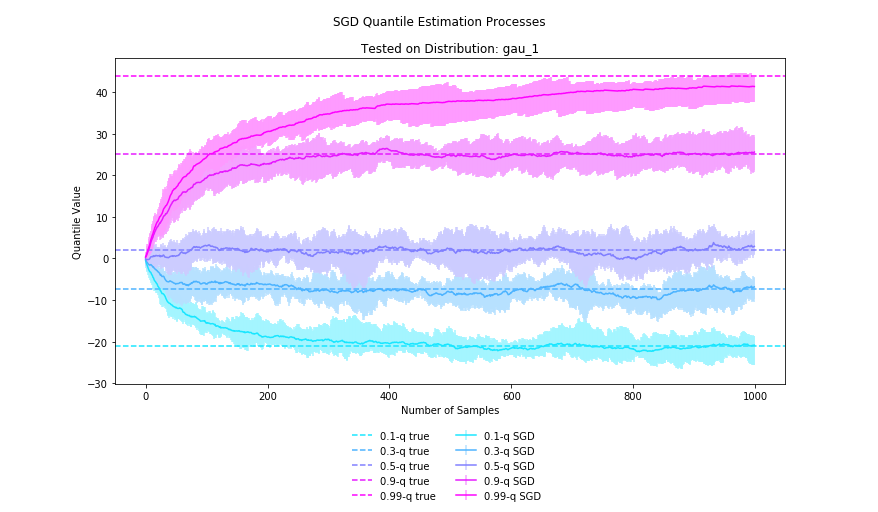
\includegraphics
    [width=1\columnwidth]
    {distro/gau_1_proc.png} % Example image
	\caption{
		SGD Process from \textit{gau-1} Distribution
    }
    \label{fig: sgd_exp_distro_gau_1_proc}
\end{figure}

\begin{figure}[H] % [h] forces the figure to be output where it is defined in the code (it suppresses floating)
	\centering
    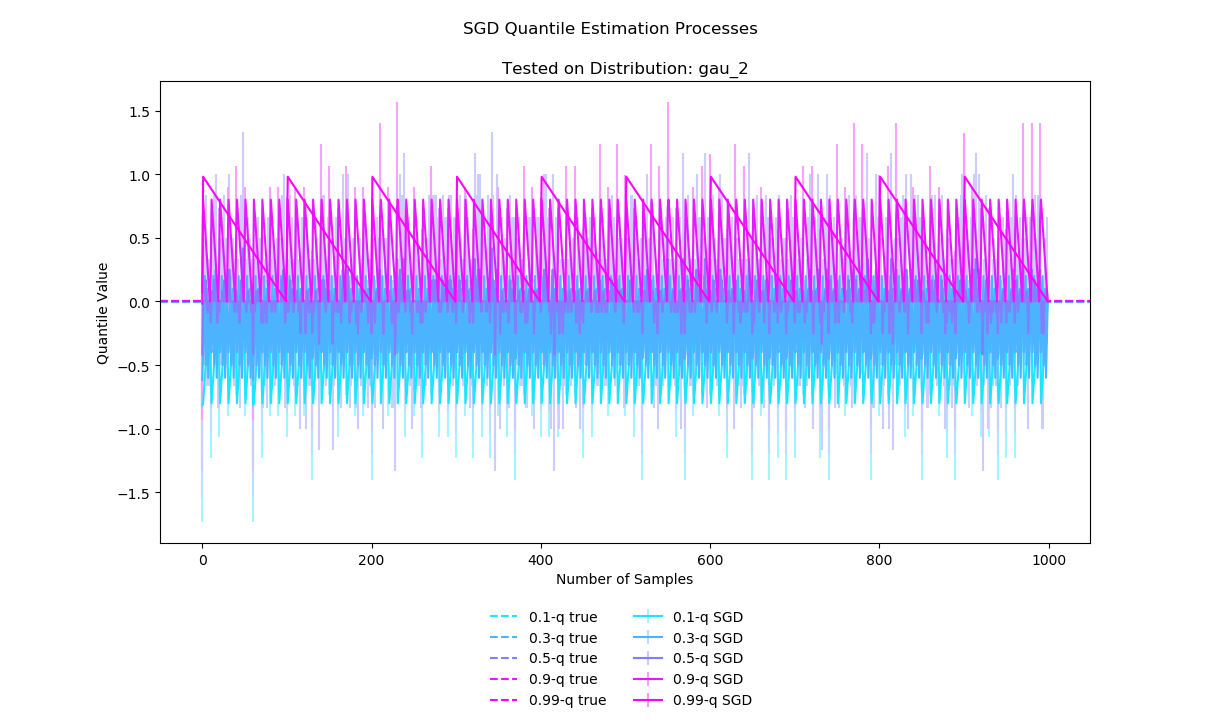
\includegraphics
    [width=1\columnwidth]
    {distro/gau_2_proc.png} % Example image
	\caption{
		SGD Process from \textit{gau-2} Distribution
    }
    \label{fig: sgd_exp_distro_gau_2_proc}
\end{figure}

\begin{figure}[H] % [h] forces the figure to be output where it is defined in the code (it suppresses floating)
	\centering
    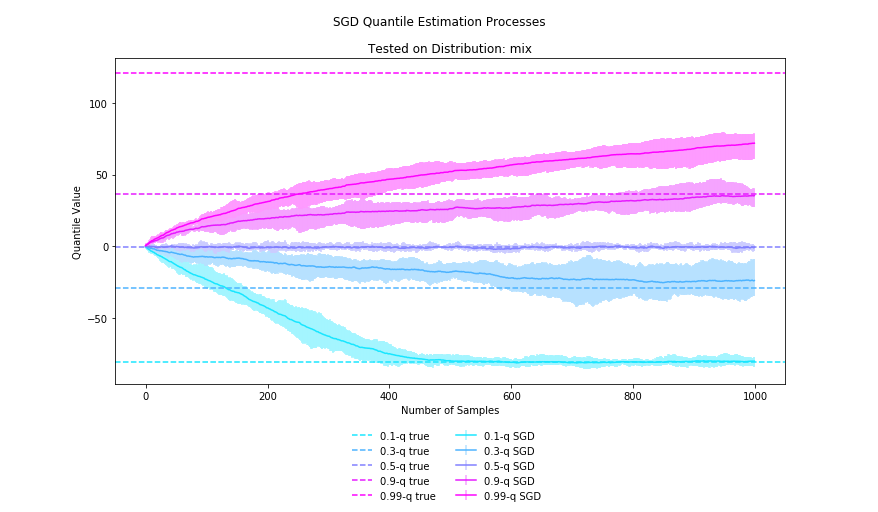
\includegraphics
    [width=1\columnwidth]
    {distro/mix_proc.png} % Example image
	\caption{
		SGD Process from \textit{mix} Distribution
    }
    \label{fig: sgd_exp_distro_mix_proc}
\end{figure}

\begin{figure}[H] % [h] forces the figure to be output where it is defined in the code (it suppresses floating)
	\centering
    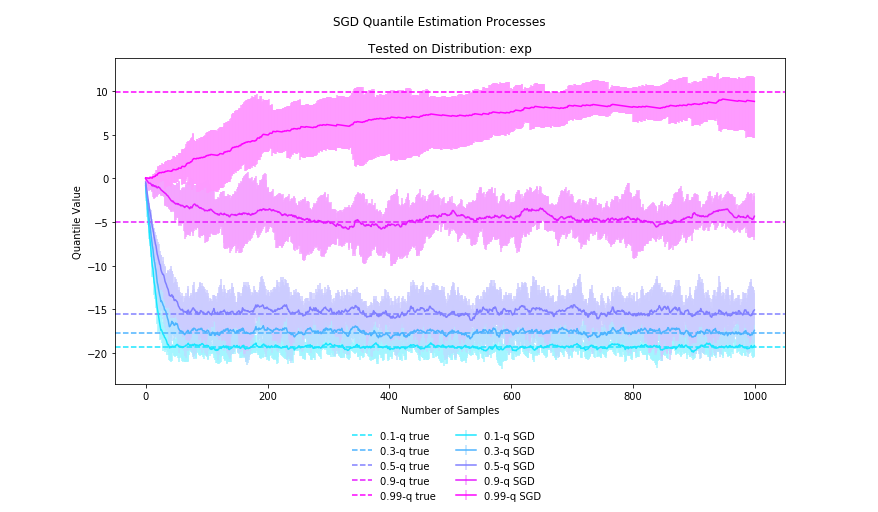
\includegraphics
    [width=1\columnwidth]
    {distro/exp_proc.png} % Example image
	\caption{
		SGD Process from \textit{exp} Distribution
    }
    \label{fig: sgd_exp_distro_exp_proc}
\end{figure}


\subsubsection{Estimate results on different distributions}
\begin{figure}[H] % [h] forces the figure to be output where it is defined in the code (it suppresses floating)
	\centering
    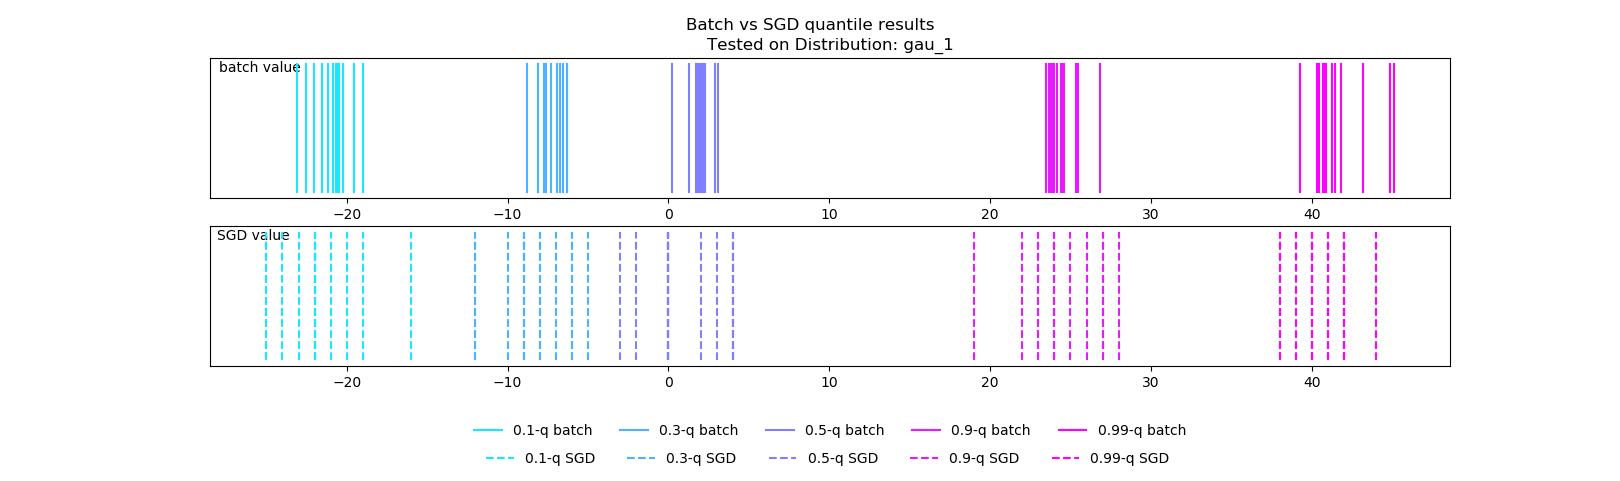
\includegraphics
    [width=1\columnwidth]
    {distro/gau_1_res.png} % Example image
	\caption{
		SGD Results from \textit{gau-1} Distribution
    }
    \label{fig: sgd_exp_distro_gau_1_res}
\end{figure}

\begin{figure}[H] % [h] forces the figure to be output where it is defined in the code (it suppresses floating)
	\centering
    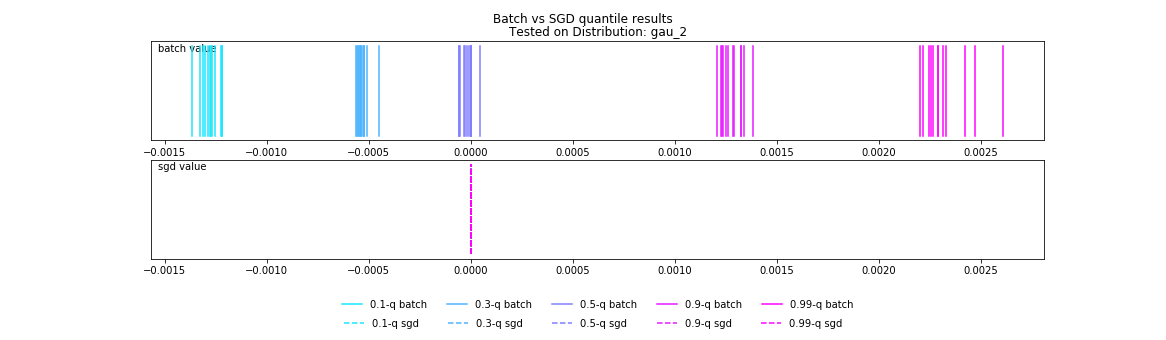
\includegraphics
    [width=1\columnwidth]
    {distro/gau_2_res.png} % Example image
	\caption{
		SGD Results from \textit{gau-2} Distribution
    }
    \label{fig: sgd_exp_distro_gau_2_res}

\end{figure}

\begin{figure}[H] % [h] forces the figure to be output where it is defined in the code (it suppresses floating)
	\centering
    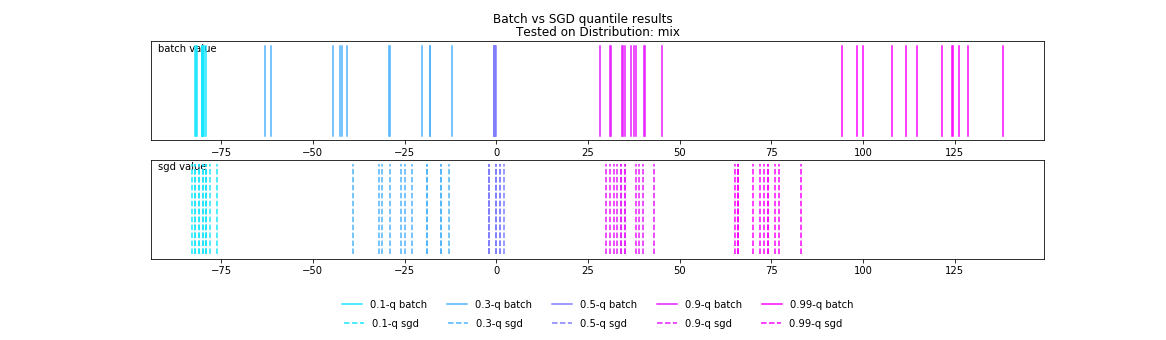
\includegraphics
    [width=1\columnwidth]
    {distro/mix_res.png} % Example image
	\caption{
		SGD Results from \textit{mix}  Distribution
	}
    \label{fig: sgd_exp_distro_mix_res}
\end{figure}

\begin{figure}[H] % [h] forces the figure to be output where it is defined in the code (it suppresses floating)
	\centering
    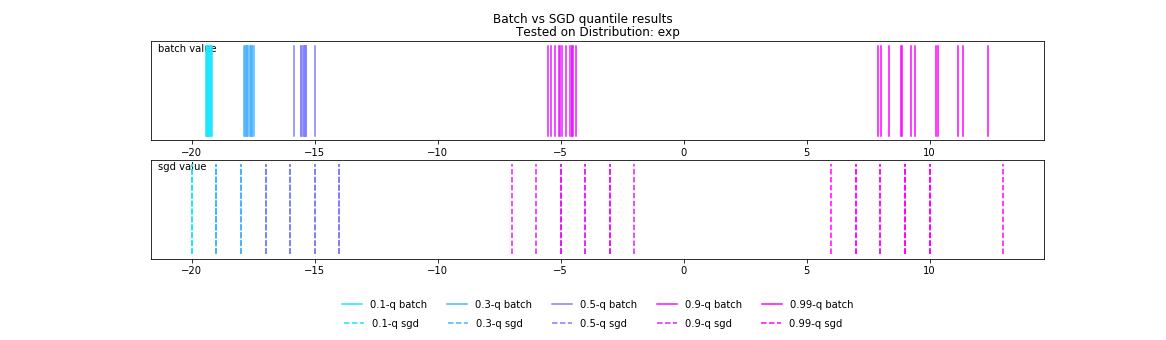
\includegraphics
    [width=1\columnwidth]
    {distro/exp_res.png} % Example image
	\caption{
		SGD Results from \textit{exp}  Distribution
	}
    \label{fig: sgd_exp_distro_exp_res}
\end{figure}

\subsubsection{Estimate Error Value on different distributions}
\begin{figure}[H] % [h] forces the figure to be output where it is defined in the code (it suppresses floating)
	\centering
    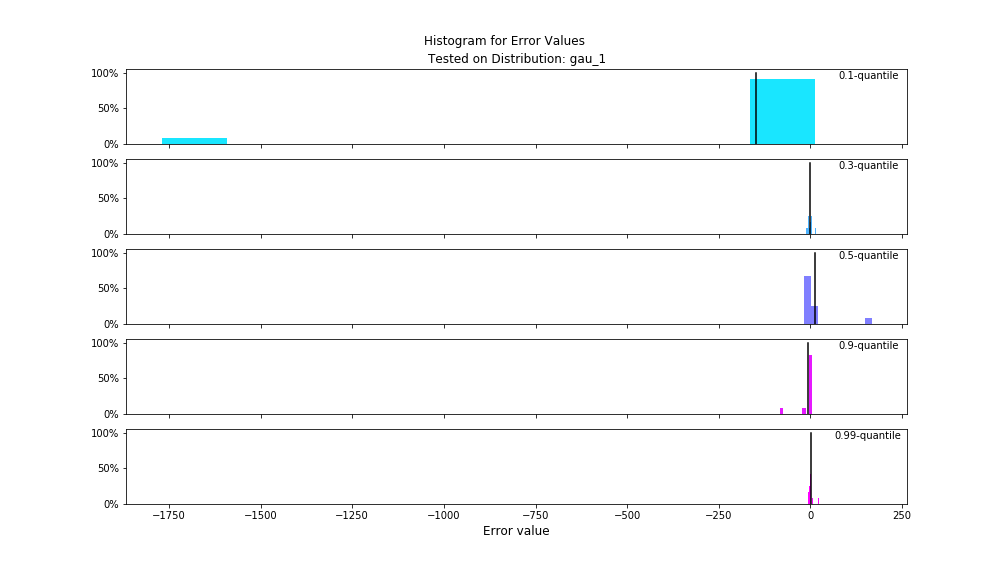
\includegraphics
    [width=1\columnwidth]
    {distro/gau_1_err.png} % Example image
	\caption{
		SGD Error from \textit{gau-1} Distribution
	}
    \label{fig: sgd_exp_distro_gau_1_err}
\end{figure}

\begin{figure}[H] % [h] forces the figure to be output where it is defined in the code (it suppresses floating)
	\centering
    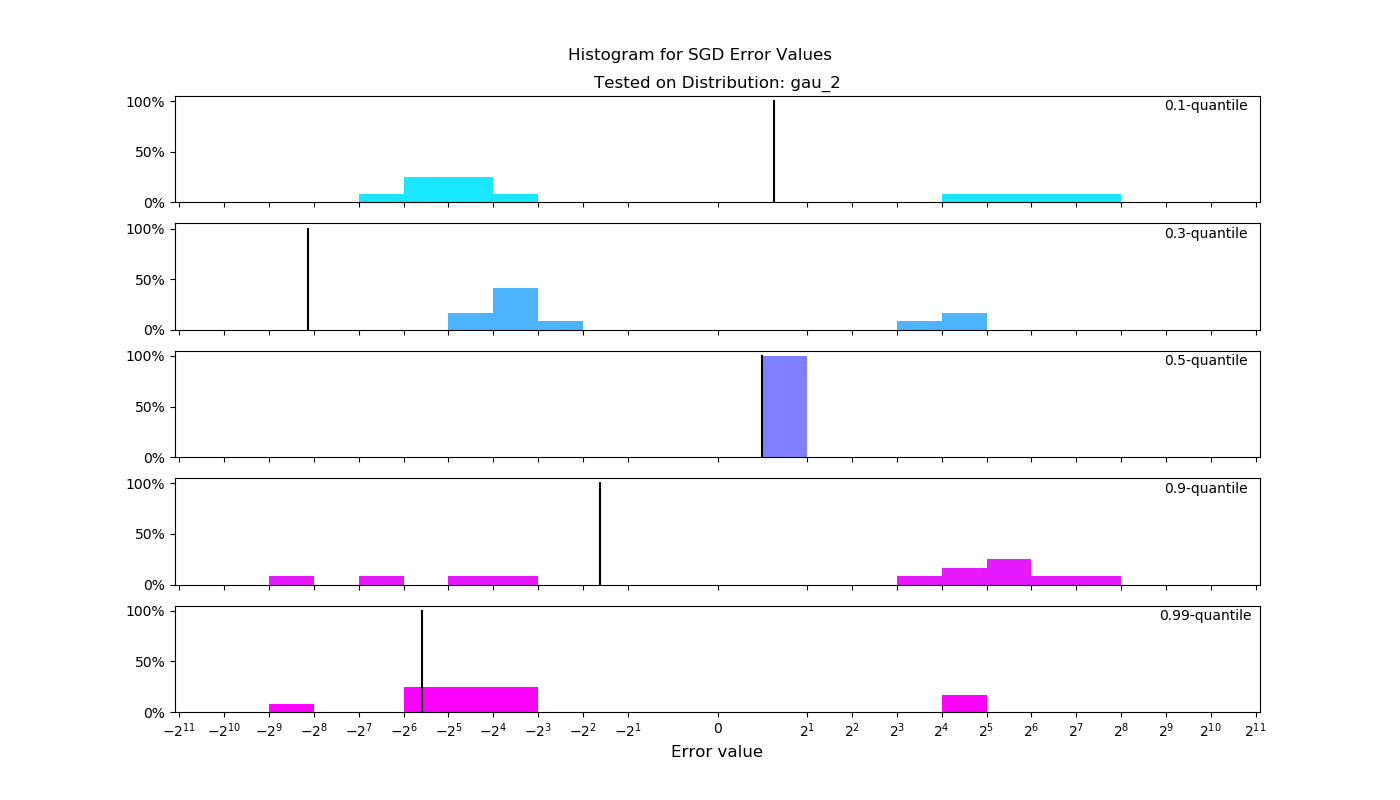
\includegraphics
    [width=1\columnwidth]
    {distro/gau_2_err.png} % Example image
	\caption{
		SGD Error from \textit{gau-2} Distribution
	}
    \label{fig: sgd_exp_distro_gau_2_err}
\end{figure}

\begin{figure}[H] % [h] forces the figure to be output where it is defined in the code (it suppresses floating)
	\centering
    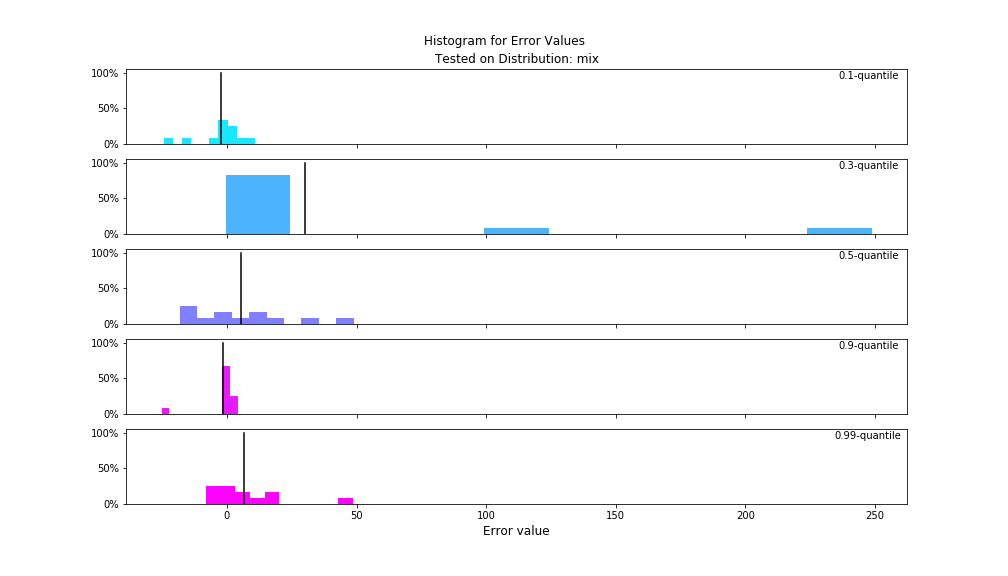
\includegraphics
    [width=1\columnwidth]
    {distro/mix_err.png} % Example image
	\caption{
		SGD Error from \textit{mix}  Distribution
	}
    \label{fig: sgd_exp_distro_mix_err}
\end{figure}

\begin{figure}[H] % [h] forces the figure to be output where it is defined in the code (it suppresses floating)
	\centering
    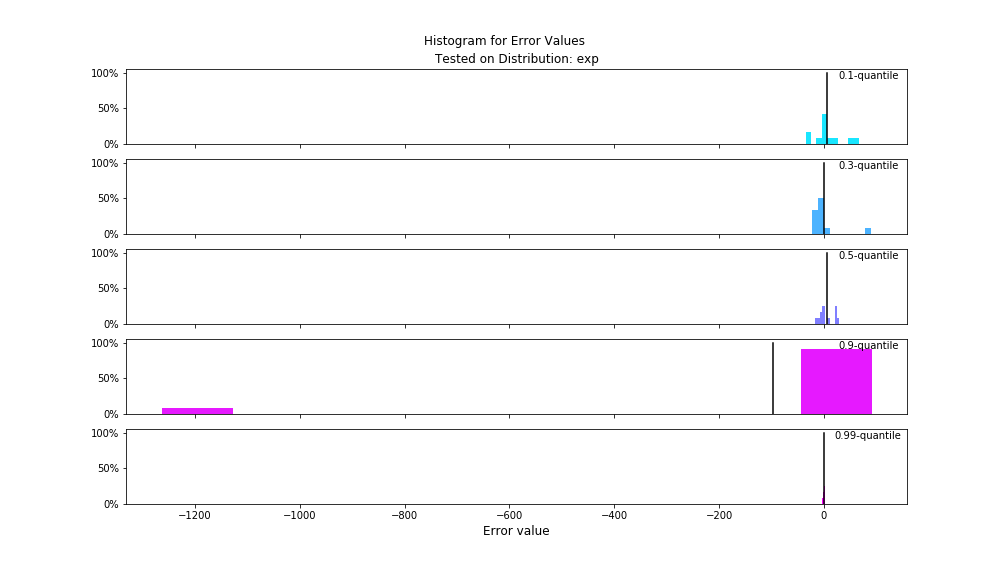
\includegraphics
    [width=1\columnwidth]
    {distro/exp_err.png} % Example image
	\caption{
		SGD Error from \textit{exp}  Distribution
	}
    \label{fig: sgd_exp_distro_exp_err}
\end{figure}

\pagebreak
\subsection{Data Size}
\label{subsec: sgd_exp_dt_size}
The experiment compares the SGD algorithm performance in 3 different data size settings: 100, 1000, 100000. In each setting, 10 data streams of the according size are generated from the \textit{gau-1} distribution, and the SGD is run on each of the data streams. The SGD algorithm is of default setting, and the performances are evaluated on the collection of the 10 SGD implementations.

The process, result and error plots for data sizes (figure~\ref{fig: sgd_exp_dt_size_100_proc} to \ref{fig: sgd_exp_dt_size_100000_err}) lead to the following interesting observations:
\begin{enumerate}
    \item Bigger data size leads to better convergence for all quantiles. When data size is 100, the $0.1, 0.9, 0.99$-q SGD are not converged to the true quantiles (figure~\ref{fig: sgd_exp_dt_size_100_proc} and \ref{fig: sgd_exp_dt_size_100_proc}), but when the size is 10 times bigger, the $0.1$ and $0.9$ quantile estimates are converged around the true values (figure~\ref{fig: sgd_exp_dt_size_1000_proc} and \ref{fig: sgd_exp_dt_size_1000_proc}) and the $0.99$-q SGD is very close to converge. When the data size reaches 100000, it is clear from figure~\ref{fig: sgd_exp_dt_size_100000_proc} that all the quantiles have converged around their corresponding true values.
    
    \item After the SGD estimates converge around the true quantiles, the fluctuation rate does not change. The "better" convergence in the last observation point refers to the stable fluctuation of quantile estimates around the true values. However, the fluctuation does not shrink after the estimate is converged. From figure \ref{fig: sgd_exp_dt_size_100000_proc} we can see the fluctuation of SGD quantile are not changed from the $20000$th epoch to the $100000$th epoch.
    
    \item Bigger data size does not mean a better effectiveness of SGD estimation. In fact, all the error values of the size 1000 SGD quantiles are better than those of the size 100000 estimates. Specifically, the former has all its error values within range $(-2^6, 2^5)$ with mean errors in range $(-2^3, 2^3)$ (figure~\ref{fig: sgd_exp_dt_size_1000_err}), while the latter has a much larger error distribution for every corresponding quantile estimate (figure~\ref{fig: sgd_exp_dt_size_100000_err}). It is because the error value is calculated as a comparison with the batch quantiles. When the data size is bigger, the batch quantiles also converges to the true quantiles, while the convergence from the SGD quantiles to the batch quantiles have not changed much. Figure~\ref{fig: sgd_exp_dt_size_1000_res} and \ref{fig: sgd_exp_dt_size_100000_res} show the batch quantiles are much denser at data size 100000, when the SGD quantiles are still distributed around them in a rather sparse way.
\end{enumerate}
\subsubsection{Estimate Processes on Different Data Size}

\begin{figure}[H] % [h] forces the figure to be output where it is defined in the code (it suppresses floating)
	\centering
    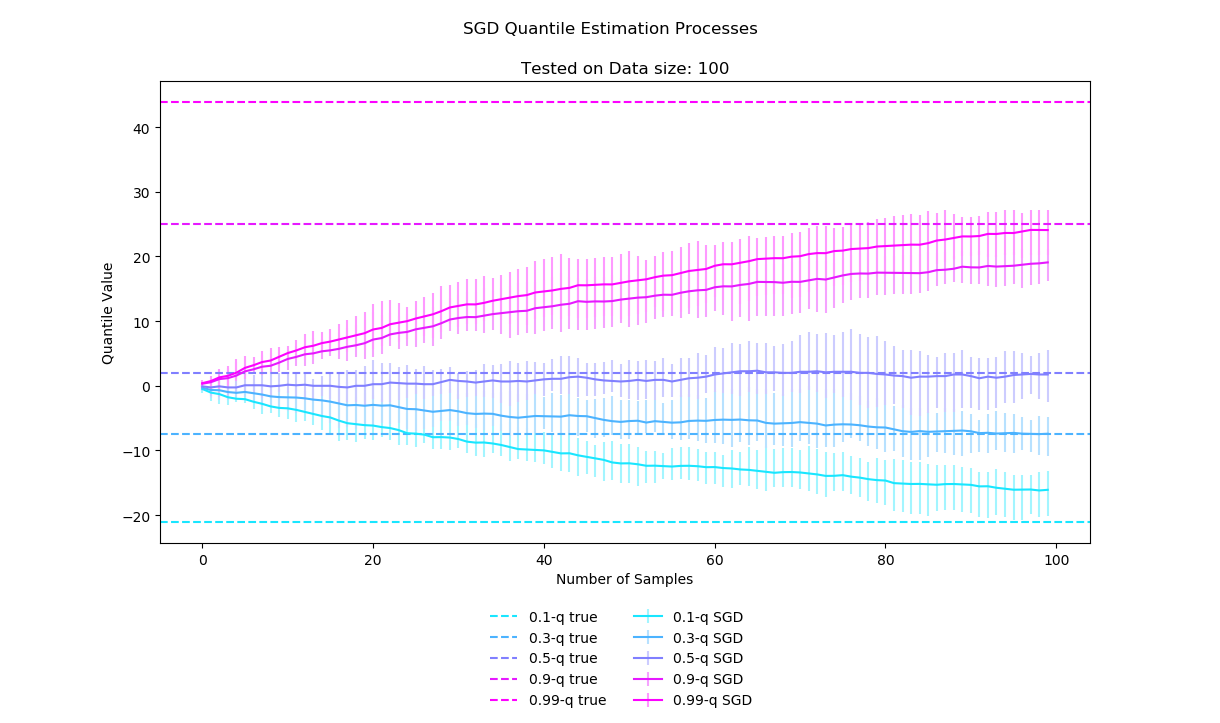
\includegraphics
    [width=1\columnwidth]
    {data_size/100_proc.png} % Example image
	\caption{
		SGD Process from 100 Samples
    }
    \label{fig: sgd_exp_dt_size_100_proc}
\end{figure}

\begin{figure}[H] % [h] forces the figure to be output where it is defined in the code (it suppresses floating)
	\centering
    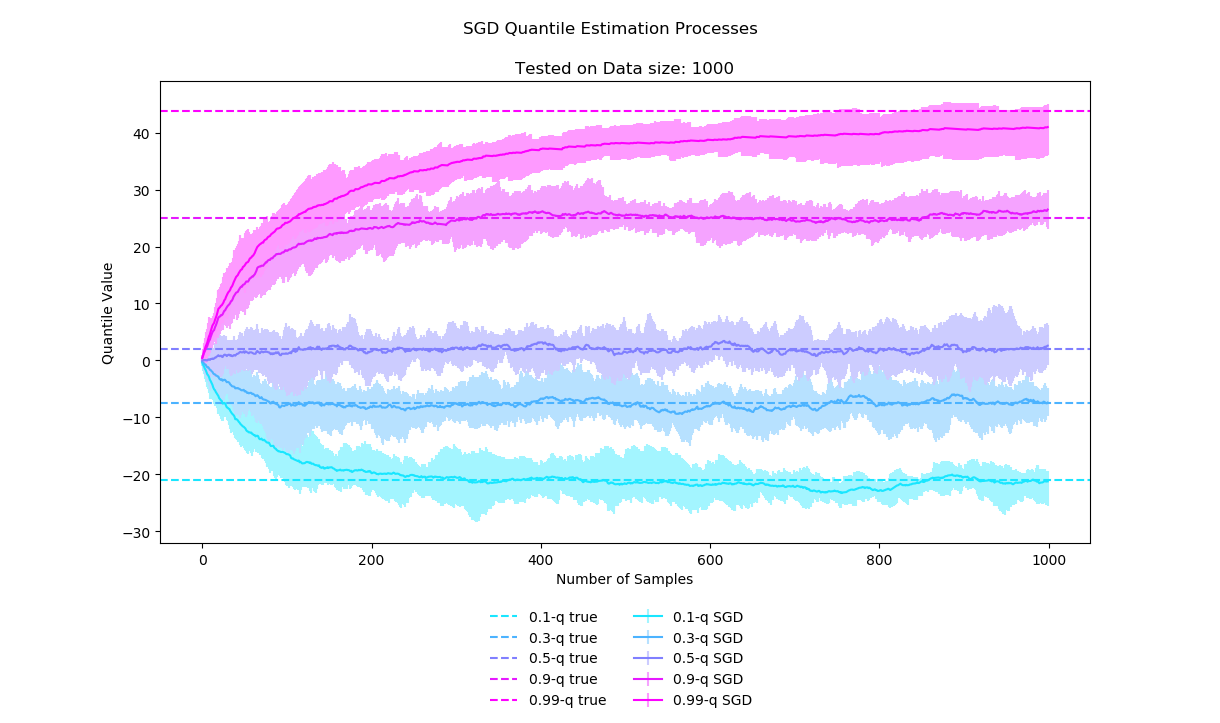
\includegraphics
    [width=1\columnwidth]
    {data_size/1000_proc.png} % Example image
	\caption{
		SGD Process from 1000 Samples
    }
    \label{fig: sgd_exp_dt_size_1000_proc}
\end{figure}
\begin{figure}[H] % [h] forces the figure to be output where it is defined in the code (it suppresses floating)
	\centering
    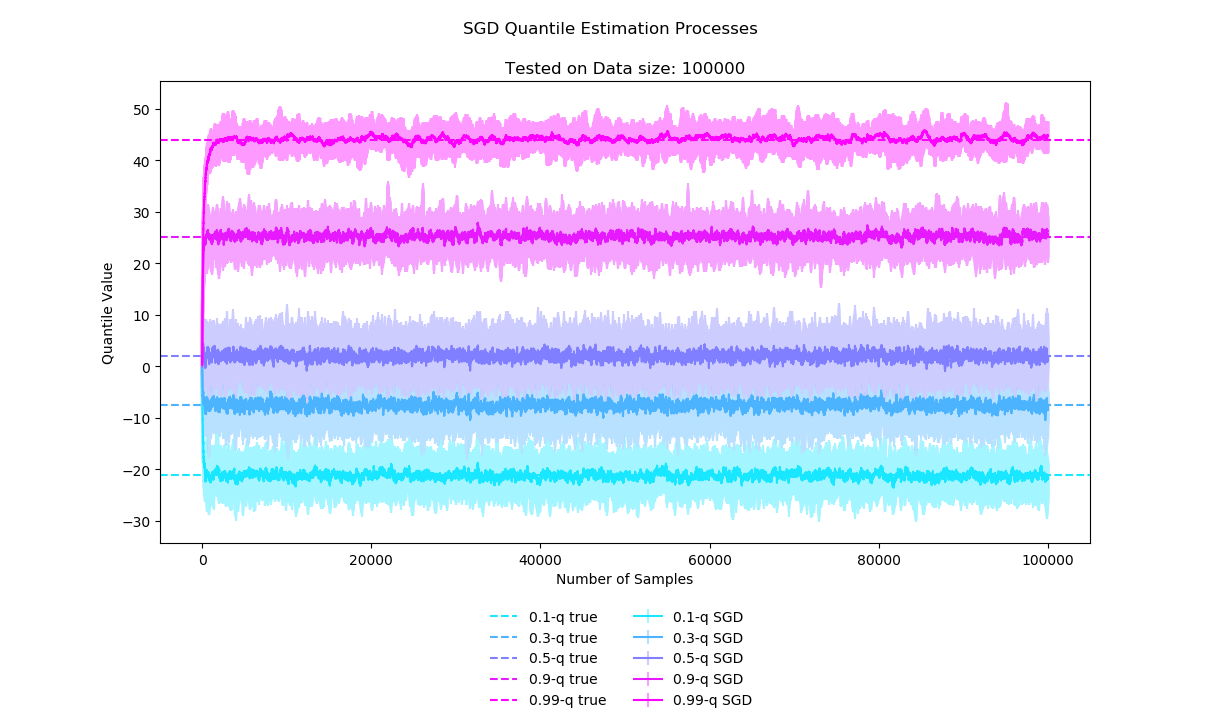
\includegraphics
    [width=1\columnwidth]
    {data_size/100000_proc.png} % Example image
	\caption{
		SGD Process from 100000 Samples
    }
    \label{fig: sgd_exp_dt_size_100000_proc}
\end{figure}

\subsubsection{Estimate Results on Different Data Size}
\begin{figure}[H] % [h] forces the figure to be output where it is defined in the code (it suppresses floating)
	\centering
    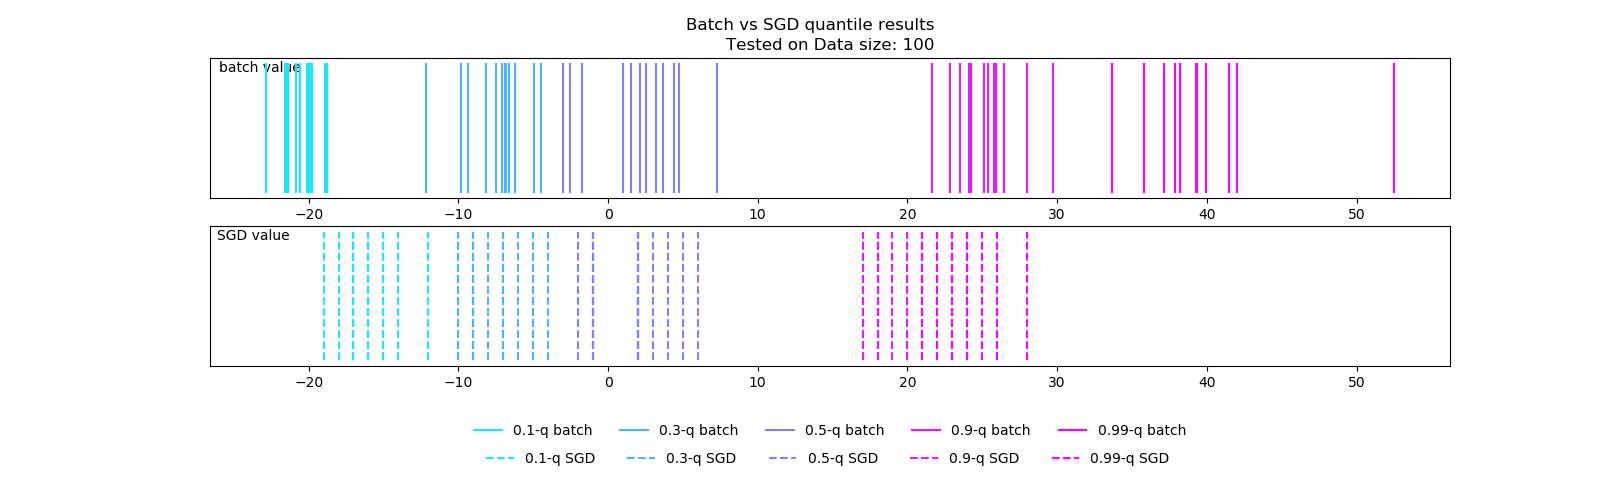
\includegraphics
    [width=1\columnwidth]
    {data_size/100_res.png} % Example image
	\caption{
		SGD Results from 100 Samples
    }
    \label{fig: sgd_exp_dt_size_100_res}
\end{figure}

\begin{figure}[H] % [h] forces the figure to be output where it is defined in the code (it suppresses floating)
	\centering
    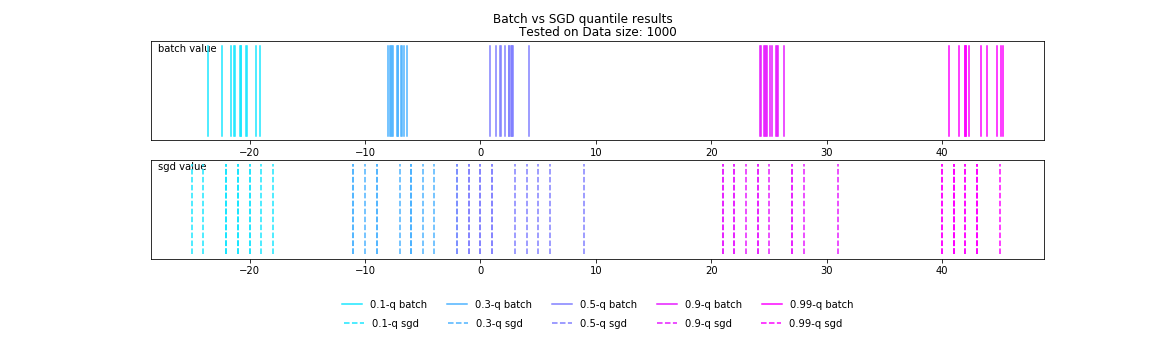
\includegraphics
    [width=1\columnwidth]
    {data_size/1000_res.png} % Example image
	\caption{
		SGD Results from 1000 Samples
	}
    \label{fig: sgd_exp_dt_size_1000_res}
\end{figure}
\begin{figure}[H] % [h] forces the figure to be output where it is defined in the code (it suppresses floating)
	\centering
    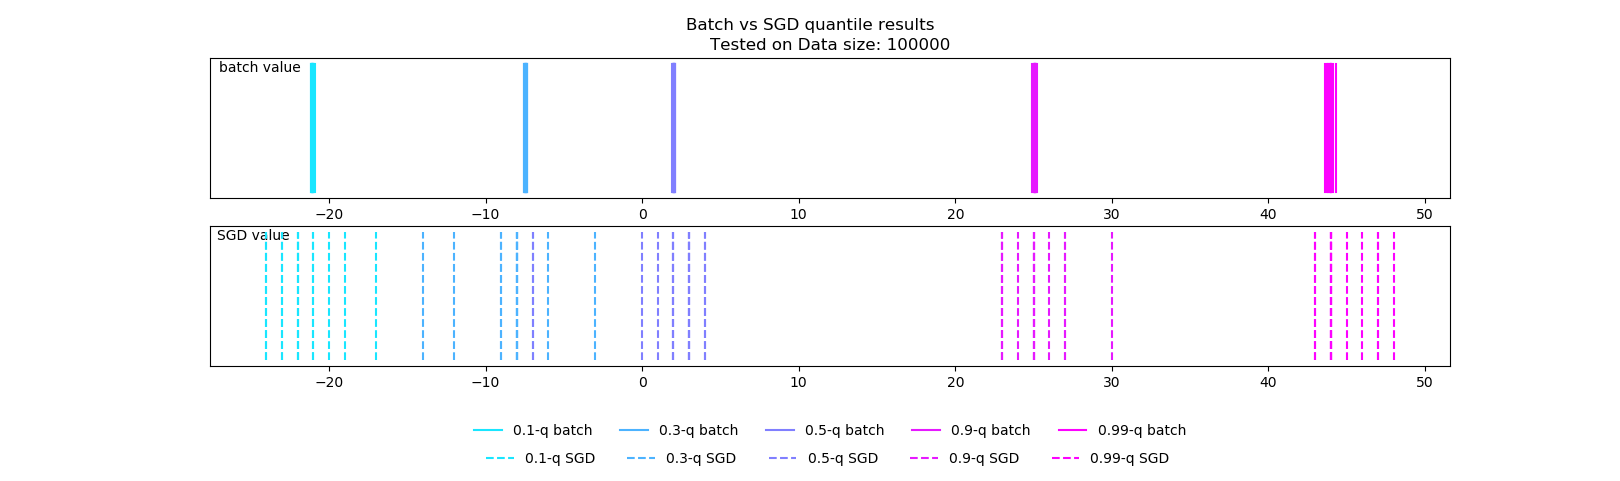
\includegraphics
    [width=1\columnwidth]
    {data_size/100000_res.png} % Example image
	\caption{
		SGD Results from 100000 Samples
	}
    \label{fig: sgd_exp_dt_size_100000_res}
\end{figure}



\subsubsection{Estimate Error Values on Different Data Size}
\begin{figure}[H] % [h] forces the figure to be output where it is defined in the code (it suppresses floating)
	\centering
    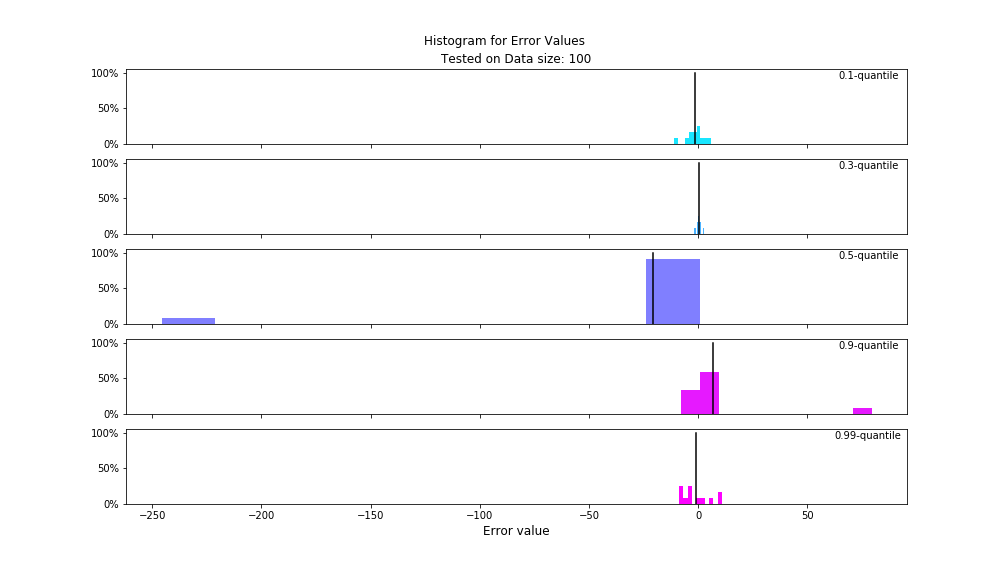
\includegraphics
    [width=1\columnwidth]
    {data_size/100_err.png} % Example image
	\caption{
		SGD Error from 100 Samples
	}
    \label{fig: sgd_exp_dt_size_100_err}
\end{figure}

\begin{figure}[H] % [h] forces the figure to be output where it is defined in the code (it suppresses floating)
	\centering
    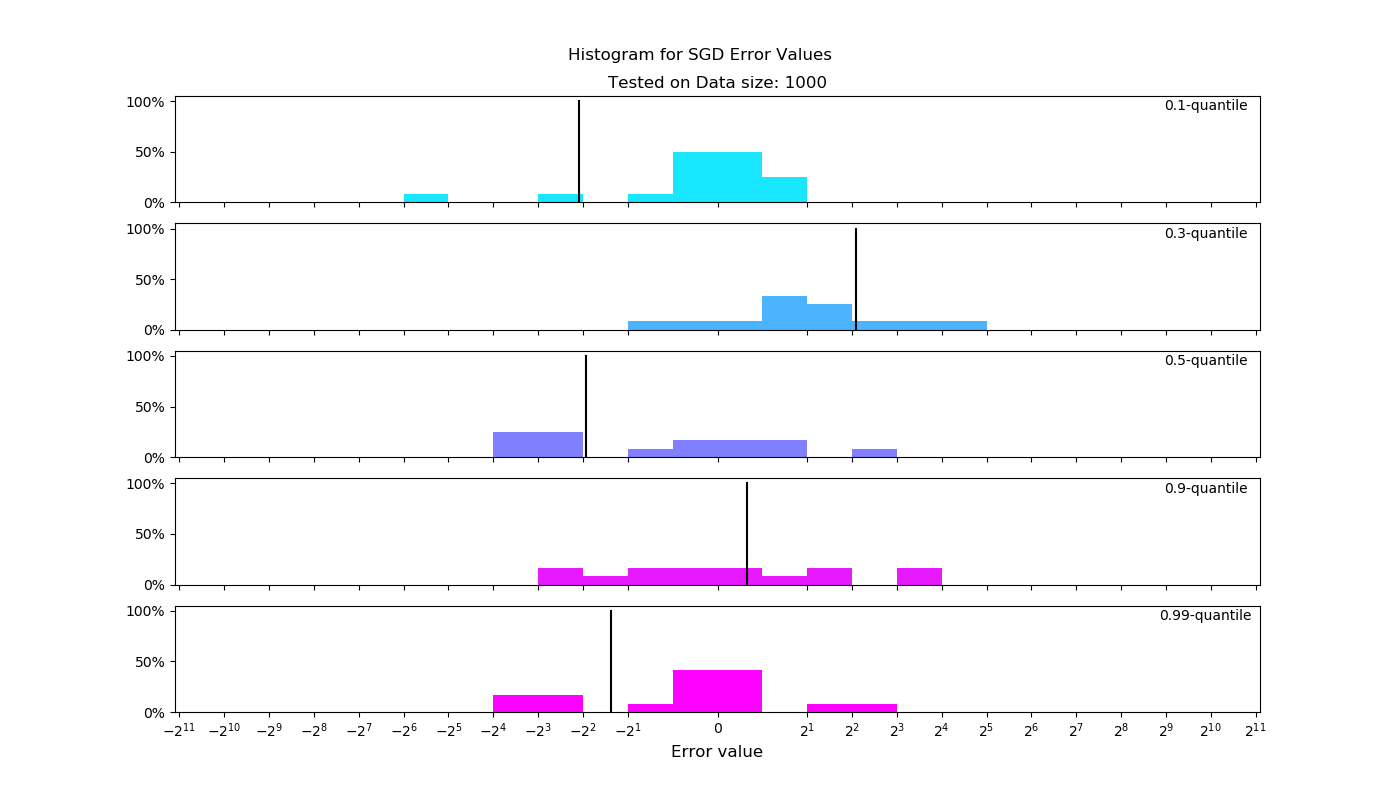
\includegraphics
    [width=1\columnwidth]
    {data_size/1000_err.png} % Example image
	\caption{
		SGD Error from 1000 Samples
	}
    \label{fig: sgd_exp_dt_size_1000_err}
\end{figure}
\begin{figure}[H] % [h] forces the figure to be output where it is defined in the code (it suppresses floating)
	\centering
    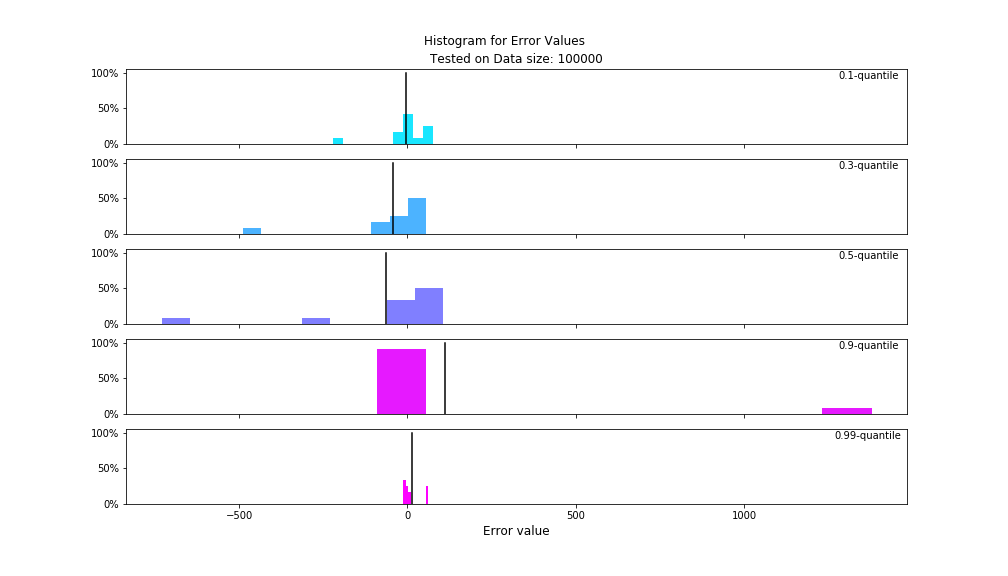
\includegraphics
    [width=1\columnwidth]
    {data_size/100000_err.png} % Example image
	\caption{
		SGD Error from 100000 Samples
	}
    \label{fig: sgd_exp_dt_size_100000_err}
\end{figure}

\pagebreak
\subsection{Ordering of Data Stream}
\label{subsec: sgd_exp_dt_ordering}
The experiment compares the SGD algorithm performance when the sequence of data stream is different. Both the data streams and the SGD algorithm are of the default settings. The experiment shuffles the same data stream 10 times, and illustrate the variance of SGD performances on those data streams. Note in this case, there is only one batch quantile value for each quantile.

The process, result and error plots for data sequence (figure~\ref{fig: sgd_exp_dt_ordering_proc} to \ref{fig: sgd_exp_dt_ordering_err}) lead to the following interesting observations:
\begin{enumerate}
    \item The impact of sequence changing is different for different quantiles. For example, the $0.99$-q SGD SGD is more densely surrounding its true quantile compared with the $0.9$-q SGD (see figure~\ref{fig: sgd_exp_dt_ordering_res} and \ref{fig: sgd_exp_dt_ordering_err}). But it is unknown if the small variance from $0.99$-q SGD is temporary or lasting. For example, the variance of the $0.1$-q SGD was very small during a short period at around the $900$th epoch, and then it get bigger again in the end(figure~\ref{fig: sgd_exp_dt_ordering_proc}).
    \item The overall affect from changing sequence does not change much of the SGD performance. All those three plots, especially figure~\ref{fig: sgd_exp_dt_ordering_err} shows that all the error values of SGD estimates are in the range $(-2^5, 2^4)$ and the mean errors are in the range ($-2^2, 2^1$). This indicates the changes in data sequence is not likely to be a big factor of SGD performances.
\end{enumerate}

\begin{figure}[H] % [h] forces the figure to be output where it is defined in the code (it suppresses floating)
	\centering
    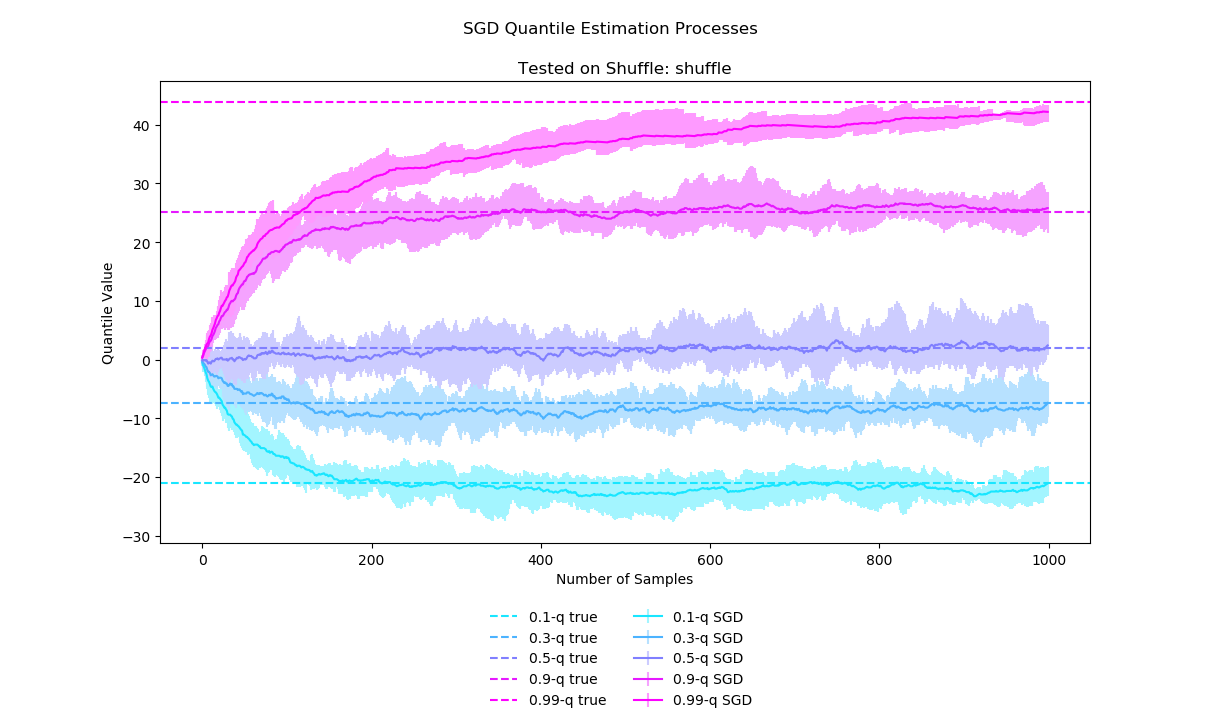
\includegraphics
    [width=1\columnwidth]
    {data_sequence/shuffle_proc.png} % Example image
	\caption{
		SGD Estimate Process from Shuffled Data Stream
    }
    \label{fig: sgd_exp_dt_ordering_proc}

\end{figure}

\begin{figure}[H] % [h] forces the figure to be output where it is defined in the code (it suppresses floating)
	\centering
    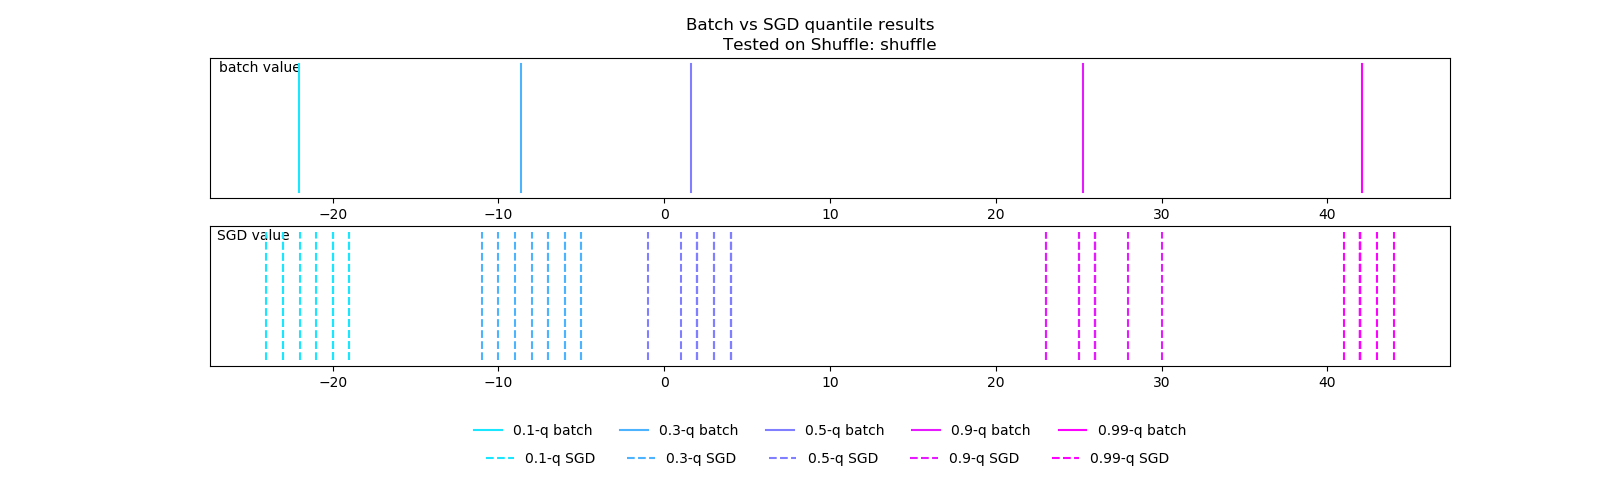
\includegraphics
    [width=1\columnwidth]
    {data_sequence/shuffle_res.png} % Example image
	\caption{
		SGD Estimate Result from Shuffled Data Stream
	}
    \label{fig: sgd_exp_dt_ordering_res}
\end{figure}

\begin{figure}[H] % [h] forces the figure to be output where it is defined in the code (it suppresses floating)
	\centering
    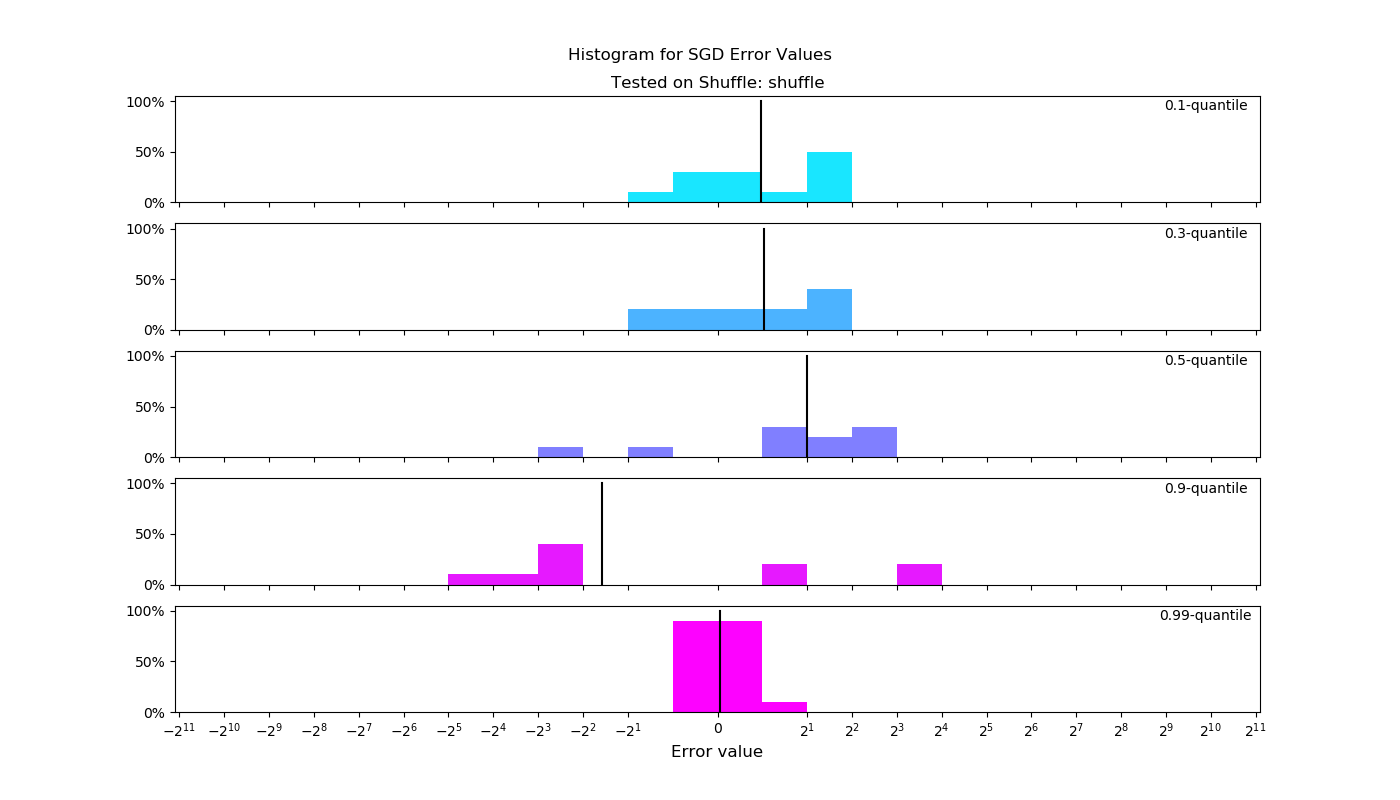
\includegraphics
    [width=1\columnwidth]
    {data_sequence/shuffle_err.png} % Example image
	\caption{
		SGD Estimate Error from Shuffled Data Stream
	}
    \label{fig: sgd_exp_dt_ordering_err}
\end{figure}

\subsection{SGD Step Size}
\label{subsec: sgd_exp_step_size}
The experiment compares the SGD algorithm performance in 3 different SGD step size settings: constant 1, diminishing $\alpha_i= \frac{2}{\sqrt{i}}$, or smaller diminishing $\alpha_i= \frac{0.002}{\sqrt{i}}$. In each setting, there are 10 data streams of the default setting, and the SGD algorithm are set at according step sizes. The performances are evaluated on the collection of the 10 SGD implementations.

The process, result and error plots for data sizes (figure~\ref{fig: sgd_exp_step_size_1_proc} to \ref{fig: sgd_exp_step_size_0002_sqrt_k_err}) lead to the following interesting observations:
\begin{enumerate}
    \item The different step sizes are different for all combinations of quantile estimation
    
    \item After convergence, the diminishing step size can improve the fluctuation problem of SGD estimates. Compared with the constant step size $\alpha_i= 1$ (figure~\ref{fig: sgd_exp_step_size_1_res}), the diminishing step size $\alpha_i= \frac{2}{\sqrt{i}}$ of the $0.5$-q SGD have both converged but the diminishing step size has a much smaller variance around the true quantile (figure~\ref{fig: sgd_exp_step_size_2_sqrt_k_res}). 
    This results in a smaller error value distribution around $0$ (figure~\ref{fig: sgd_exp_step_size_2_sqrt_k_err}), which means a more accurate estimation.

    \item The small error distribution range with mean close to 0 cannot not imply to a good convergence. When $\alpha_i= \frac{0.002}{\sqrt{i}}$, the mean error value of the $0.5$-q SGD is in $(0,1)$, and the error discussion lies in a small range of $(-2^3, 2^5)$ (figure~\ref{fig: sgd_exp_step_size_0002_sqrt_k_err}), however, it is clear in both the process and result figures (figure~\ref{fig: sgd_exp_step_size_0002_sqrt_k_proc} and \ref{fig: sgd_exp_step_size_0002_sqrt_k_res}) that the SGD estimate does not move much towards the true quantile value at 2. The corresponding reflection on the error plot is that the error values are never within the range $(-2^2, 2^2)$, suggesting that the mean error is just a balance between two groups of big errors on both side. 
\end{enumerate}
\subsubsection{Estimate Processes on Different SGD Step sizes}
\begin{figure}[H] % [h] forces the figure to be output where it is defined in the code (it suppresses floating)
	\centering
    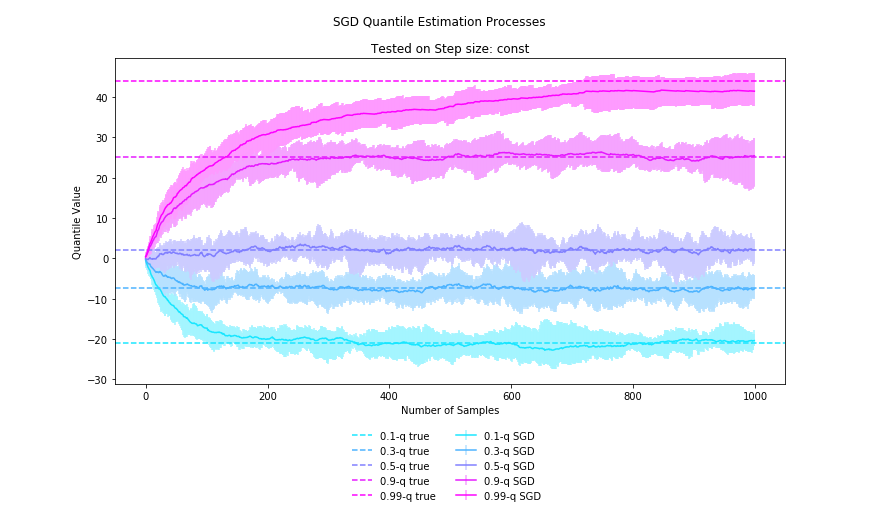
\includegraphics
    [width=1\columnwidth]
    {step_size/const_proc.png} % Example image
	\caption{
		SGD Estimate Process from step size $\alpha_i =1 $
    }
    \label{fig: sgd_exp_step_size_1_proc}

\end{figure}

\begin{figure}[H] % [h] forces the figure to be output where it is defined in the code (it suppresses floating)
	\centering
    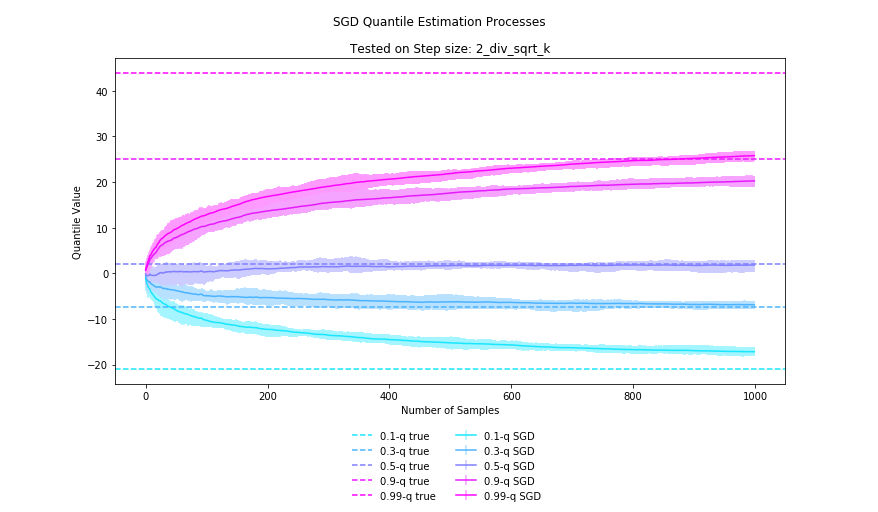
\includegraphics
    [width=1\columnwidth]
    {step_size/2_div_sqrt_k_proc.png} % Example image
	\caption{
		SGD Estimate Process from step size $ \alpha_i = \frac{2}{\sqrt{i}}$
	}
    \label{fig: sgd_exp_step_size_2_sqrt_k_proc}
\end{figure}

\begin{figure}[H] % [h] forces the figure to be output where it is defined in the code (it suppresses floating)
	\centering
    \includegraphics
    [width=1\columnwidth]
    {step_size/{0.002_div_sqrt_k_proc}.png} % Example image
	\caption{
		SGD Estimate Process from step size $ \alpha_i = \frac{0.002}{\sqrt{i}}$
	}
    \label{fig: sgd_exp_step_size_0002_sqrt_k_proc}
\end{figure}

\subsubsection{Estimate Results on Different SGD Step sizes}
\begin{figure}[H] % [h] forces the figure to be output where it is defined in the code (it suppresses floating)
	\centering
    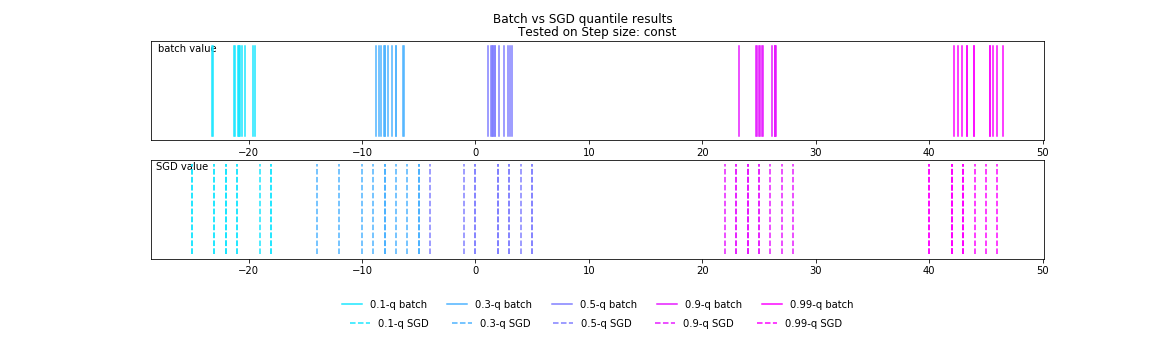
\includegraphics
    [width=1\columnwidth]
    {step_size/const_res.png} % Example image
	\caption{
		SGD Estimate Results from step size $\alpha_i =1 $
	}
    \label{fig: sgd_exp_step_size_1_res}
\end{figure}

\begin{figure}[H] % [h] forces the figure to be output where it is defined in the code (it suppresses floating)
	\centering
    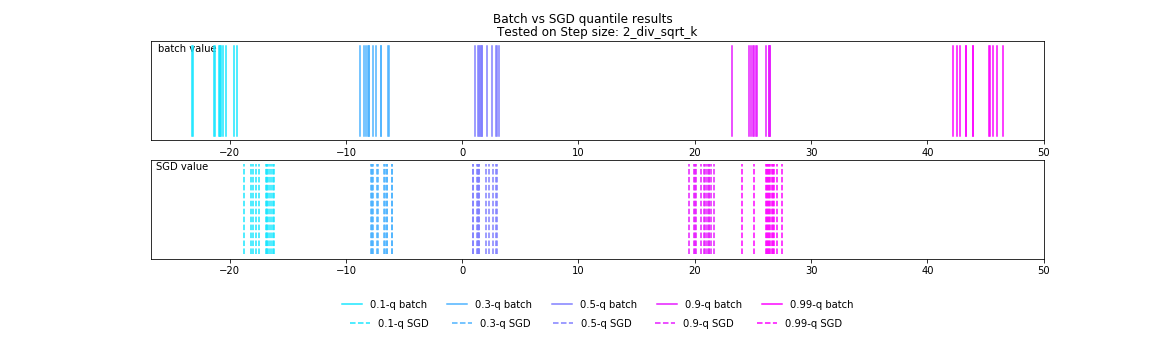
\includegraphics
    [width=1\columnwidth]
    {step_size/2_div_sqrt_k_res.png} % Example image
	\caption{
		SGD Estimate Results from step size $ \alpha_i = \frac{2}{\sqrt{i}}$
	}
    \label{fig: sgd_exp_step_size_2_sqrt_k_res}
\end{figure}

\begin{figure}[H] % [h] forces the figure to be output where it is defined in the code (it suppresses floating)
	\centering
    \includegraphics
    [width=1\columnwidth]
    {step_size/{0.002_div_sqrt_k_res}.png} % Example image
	\caption{
		SGD Estimate Results from step size $ \alpha_i = \frac{0.002}{\sqrt{i}}$
	}
    \label{fig: sgd_exp_step_size_0002_sqrt_k_res}
\end{figure}

\subsubsection{Estimate Error Values on Different SGD Step sizes}
\begin{figure}[H] % [h] forces the figure to be output where it is defined in the code (it suppresses floating)
	\centering
    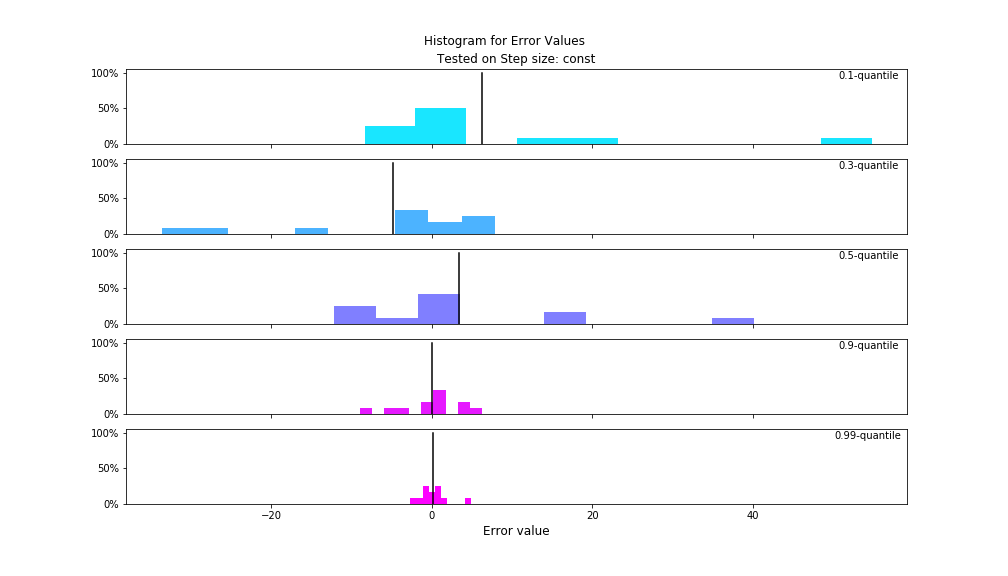
\includegraphics
    [width=1\columnwidth]
    {step_size/const_err.png} % Example image
	\caption{
		SGD Estimate Error from step size $\alpha_i =1 $
	}
    \label{fig: sgd_exp_step_size_1_err}
\end{figure}

\begin{figure}[H] % [h] forces the figure to be output where it is defined in the code (it suppresses floating)
	\centering
    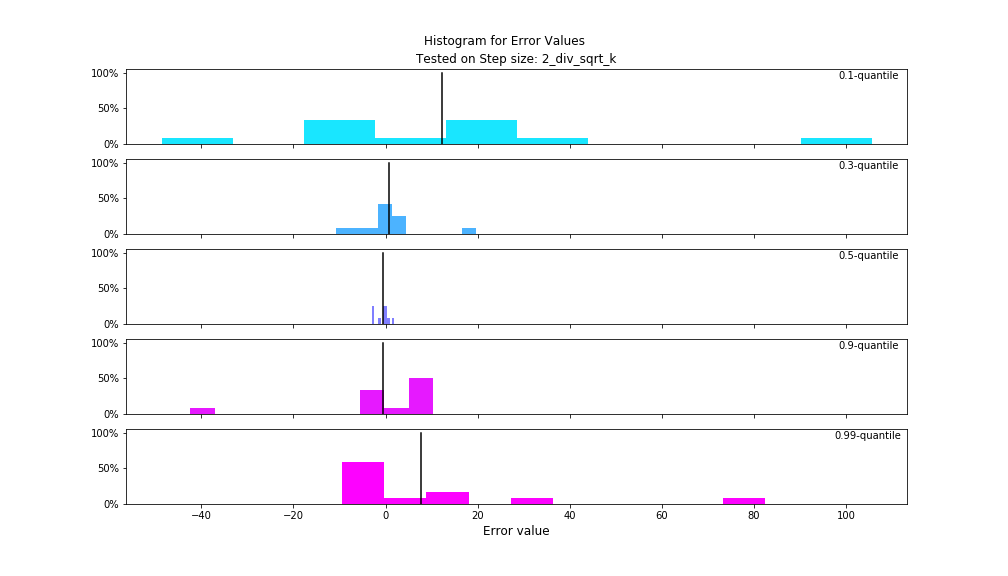
\includegraphics
    [width=1\columnwidth]
    {step_size/2_div_sqrt_k_err.png} % Example image
	\caption{
		SGD Estimate Error from step size $ \alpha_i = \frac{2}{\sqrt{i}}$
	}
    \label{fig: sgd_exp_step_size_2_sqrt_k_err}
\end{figure}

\begin{figure}[H] % [h] forces the figure to be output where it is defined in the code (it suppresses floating)
	\centering
    \includegraphics
    [width=1\columnwidth]
    {step_size/{0.002_div_sqrt_k_err}.png} % Example image
	\caption{
		SGD Estimate Error from step size $ \alpha_i = \frac{0.002}{\sqrt{i}}$
	}
    \label{fig: sgd_exp_step_size_0002_sqrt_k_err}
\end{figure}

\pagebreak
\section{Discussion}
\label{sec: discussion}
\subsection{SGD step sizes and distributions}

The selection of appropriate step sizes for different distributions is of great importance. The impact of excessively small step sizes on a distribution is shown in section~\ref{subsec: sgd_exp_step_size}. The extreme case with overly big step size, on the other hand, is illustrated from the weird performance of SGD in the \textit{gau-2} distributions (see subsection~\ref{subsec: sgd_exp_distro}).

The uncommon performance of it is reflected in all the three aspects of process, results and error values. For example, we notice the regular sawtooth update line of the $0.99$-q SGD in figure~\ref{fig: sgd_exp_distro_gau_2_proc}. The mechanism of $0.99$-q SGD is that it increase by $0.99$ when observe a data greater than the current estimate, and decrease by $0.01$ otherwise. Note in \textit{gau-2}, the probability of sampling a data outside $(-0.01, 0.01)$ is close to 0. This means, the initialization estimate at 0 is highly likely to lead to an increase of $0.99$ in the first or the second epoch. Once the quantile estimate is beyond the range $(-0.01, 0.01)$, the next data is nearly impossible to be a bigger one, so the estimate decreases with possibility close to 1. Which is why the $0.99$-q SGD decrease by $0.01$ until it reaches 0 again. The round of "start from 0, (maybe decrease a bit,) increase for one iteration, then decrease back to 0" takes exactly 100 epochs. So the results of the $0.99$-q SGD nearly always ends up at 0 after 1000 epochs. The other quantiles face with the similar problem, so they are also very likely to reach exactly 0 after 1000 epochs. This explains why in figure~\ref{fig: sgd_exp_distro_gau_2_res} all SGD estimates are in the same value $0$. 

The choice of step size is not only important for SGD on quantile estimation, but is also a popular topic for general SGD methods in machine learning. In chapter~\ref{ch: SAG}, we provide some further discussions on the adaptation of step size for different data streams inspired by the current machine learning methods.

\subsection{SGD step size and data size}

There is no experiment showing the relationship between SGD step size and dataset size, but the process figure of step size $\alpha_i = \frac{2}{\sqrt{i}}$ (figure~\ref{fig: sgd_exp_step_size_2_sqrt_k_proc}) shows the trend of $0.9$ and $0.1$-q SGD are approaching their true quantile, and it is likely that the convergence can be reached in another 1000 epochs. For the $0.99$-q SGD however, the convergence trend will be much longer than 1000 epochs for it is further away from the true quantile and the slope of the trend is low.

The convergence issue of step size $\alpha_i = \frac{0.002}{\sqrt{i}}$ can hardly be solved by the expansion of data stream size. From figure~\ref{fig: sgd_exp_step_size_0002_sqrt_k_proc} we can see the slow SGD update trend for all quantiles are almost flat. Under the condition that the step sizes are diminishing, it highly possible that the convergence would not happen for any quantiles even if the data is 100 times bigger.

\subsection{Starting point and the convergence}

The starting point of SGD is another interesting variable of SGD algorithm, but it is not investigated in this chapter. For example, in the experiment that the SGD step size is $\alpha_i = \frac{0.002}{\sqrt{i}}$ for the $gau-1$ distribution, if the initialization of the $0.5$-q SGD starts at $1.9$ instead of $0$ (the true $0.5$-q $=2$), then the SGD will have a much accurate estimation.

An optimal choice of initialization is obviously the true quantile. And a feasible good option is to have the initialization quantile estimate at the position close to the true quantile. An easy solution is to sort the first few data points and use the batch quantile of this group of small samples as initialization. This is a potential further improvement direction for our SGD quantile estimation research.

\section{Conclusion}
In this chapter, we conduct experiments on SGD for quantile estimation. We find that the performance of the algorithm are affected by the input data stream as well as the variable setting in SGD. For data streams, the changes in data distribution, data size and data sequence all affect the performances of SGD. Specifically, the SGD works well when
\begin{itemize}
    \item The true quantiles in the data distribution are well-distributed. If it is too far from the initial quantile estimate, the convergence cannot be reached by SGD within the given number of epochs (e.g., the $0.99$-q for \textit{gau-1}).
    At the same time, the true quantile should not be too close to each other. Otherwise 
    the quantile estimates are likely to violate the monotone property, and additionally the low precision can be pointless for the estimation result (e.g., all quantiles in \textit{gau-2}). 
    
    \item The data size is not too small for the SGD quantiles to converge (e.g., the $0.99$-q for data size = 100), and the same time not too big so that the precision of SGD estimation is close to the batch quantiles (e.g., all quantiles for data size = 100000)
    
    \item The data sequence is of any ordering. The ordering of data sequence does not have a big impact on the performance, but this conclusion needs to be checked with more empirical experiments or mathematical explanations.
    
    \item The step size of SGD is big enough for a convergence, and the fluctuation can decrease when it reaches the convergence (e.g., the $0.3$-q for diminishing step size $\alpha_i = \frac{2}{\sqrt{i}}$).
\end{itemize}

Besides these observations, we believe the combination effect of different settings can also work together. For example, the problem of small step size can sometimes be solved by a double size of the data stream. It is also mentioned that the initialization of SGD quantiles can be another contributing variable for the estimation performance. 

Since the properties of data stream is unknown to the algorithm, the only improvement direction for SGD is to change its settings so it works better in different conditions. In the following chapters, we explore the improvement of SGD on two problems: the crossing quantile estimates and the adaptation of step size. In chapter~\ref{ch: multi_quant} we look into potential solutions to keep the monotone properties, and in chapter~\ref{ch: SAG} we introduce our new method for step size adaptation.
% \end{document}
% \end(documentclass)